\documentclass[11pt,a4paper]{article}

% --- Packages ---
\usepackage[utf8]{inputenc}
\usepackage[margin=1in]{geometry}
\usepackage{titlesec}
\usepackage{hyperref}
\usepackage{booktabs}
\usepackage{tabularx}
\usepackage{amsmath,amssymb}
\usepackage{graphicx}
\usepackage{xcolor}
\usepackage{listings}
\usepackage{tikz}
\usetikzlibrary{shapes.geometric, arrows.meta, positioning, calc, fit, backgrounds, shadows}
\usepackage{enumitem}
\usepackage{fancyhdr}

% --- Colors ---
\definecolor{primary}{RGB}{30, 58, 138}     % Deep Blue
\definecolor{secondary}{RGB}{14, 116, 144}  % Cyan/Teal
\definecolor{accent}{RGB}{217, 119, 6}     % Amber
\definecolor{danger}{RGB}{185, 28, 28}     % Crimson
\definecolor{darkgray}{RGB}{51, 65, 85}
\definecolor{lightgray}{RGB}{241, 245, 249}
\definecolor{codebg}{RGB}{248, 250, 252}

% --- Hyperref Setup ---
\hypersetup{
    colorlinks=true,
    linkcolor=primary,
    filecolor=secondary,      
    urlcolor=primary,
    citecolor=primary
}

% --- Typography & Spacing ---
\setlength{\parindent}{0pt}
\setlength{\parskip}{6pt plus 2pt minus 1pt}

% --- Header and Footer ---
\pagestyle{fancy}
\fancyhf{}
\rhead{\textcolor{darkgray}{\footnotesize Solwin ML Services Architecture \& System Design}}
\lhead{\textcolor{darkgray}{\footnotesize Technical Design Document}}
\rfoot{\thepage}
\renewcommand{\headrulewidth}{0.4pt}
\renewcommand{\footrulewidth}{0.4pt}

% --- Code Listing Setup ---
\lstset{
    backgroundcolor=\color{codebg},
    basicstyle=\ttfamily\footnotesize\color{darkgray},
    breakatwhitespace=false,
    breaklines=true,
    captionpos=b,
    keepspaces=true,
    numbers=left,
    numbersep=5pt,
    numberstyle=\tiny\color{gray},
    showspaces=false,
    showstringspaces=false,
    showtabs=false,
    tabsize=2,
    frame=single,
    rulecolor=\color{lightgray}
}

% ==============================================================================
% DOCUMENT BEGINS
% ==============================================================================
\begin{document}

% --- Title Block ---
\begin{center}
    {\LARGE \textbf{\color{primary} Solwin ML Services Architecture \& System Design}}\\[6pt]
    {\large High-Throughput Hybrid Intelligence, Security Defense, and Decision Routing}\\[4pt]
    \vspace{2pt}
    \textbf{Version:} 1.2.0 \quad \textbar \quad \textbf{System Tier:} ML Microservices (Port 8000) \quad \textbar \quad \textbf{Status:} Production Refined\\[1pt]
    \textbf{Author:} Solwin Core Intelligence Engineering Team\\[8pt]
    \rule{\linewidth}{1pt}
\end{center}

\begin{abstract}
This system design document details the architecture, component topology, failure modes, data contracts, and algorithmic foundations of the \textbf{Solwin ML Service} (\texttt{app/ml\_services}). Solwin operates as a dual-engine platform combining fast, deterministic local inference (sub-5ms CPU heuristics, TF-IDF category classification, and regex security scanners) with cloud-native generative AI models (Google Gemini 2.5 Flash). The service delivers automated complaint classification across 11 canonical business sectors, unsupervised centroid clustering, objective urgency calculation, factual resolution state tracking, URL/email security threat intelligence, zero-hallucination entity summarization, and rule-governed operational routing.
\end{abstract}

\tableofcontents
\vspace{1em}
\hrule
\vspace{1.5em}

% ==============================================================================
\section{Executive Summary \& Design Objectives}
% ==============================================================================
Customer support queues are frequently flooded with unstructured, noisy, and high-velocity tickets. Conventional triage relies on human agents or naive keyword heuristics that suffer from two critical vulnerabilities:
\begin{enumerate}[leftmargin=*]
    \item \textbf{Inconsistent Security Detection:} Evolving social engineering lures, credential manipulation, punycode spoofing, and obscured shorteners bypass static rules.
    \item \textbf{Time-Consuming Operational Latency:} Manually scanning URLs, checking domain registries, evaluating business urgency, and synthesizing message threads causes massive SLA breaches.
\end{enumerate}

The Solwin ML Service solves these challenges through a \textbf{Hybrid Tier Architecture}:
\begin{itemize}[leftmargin=*]
    \item \textbf{Ultra-Low Latency Deterministic Core:} Runs on edge/standard CPU runtimes without external dependencies to deliver sub-5ms classification, URL threat parsing, domain typosquat detection, and action routing.
    \item \textbf{High-Order Semantic AI Layer:} Orchestrates Google Gemini 2.5 Flash via structured JSON schema enforcement for nuanced social engineering detection, sentiment analysis, and abstractive entity summarization.
    \item \textbf{Zero Downtime Fallback Matrix:} When cloud AI endpoints encounter rate limits (HTTP 429), timeouts, or network outages, the pipeline deterministically falls back to local calibrated estimators and flags records with \texttt{needs\_review = true}.
\end{itemize}

% ==============================================================================
\section{High-Level System Architecture}
% ==============================================================================
The ML Service operates inside an isolated, non-root, read-only multi-stage container exposing high-performance asynchronous REST endpoints on \textbf{Port 8000}.

\begin{figure}[htbp]
\centering
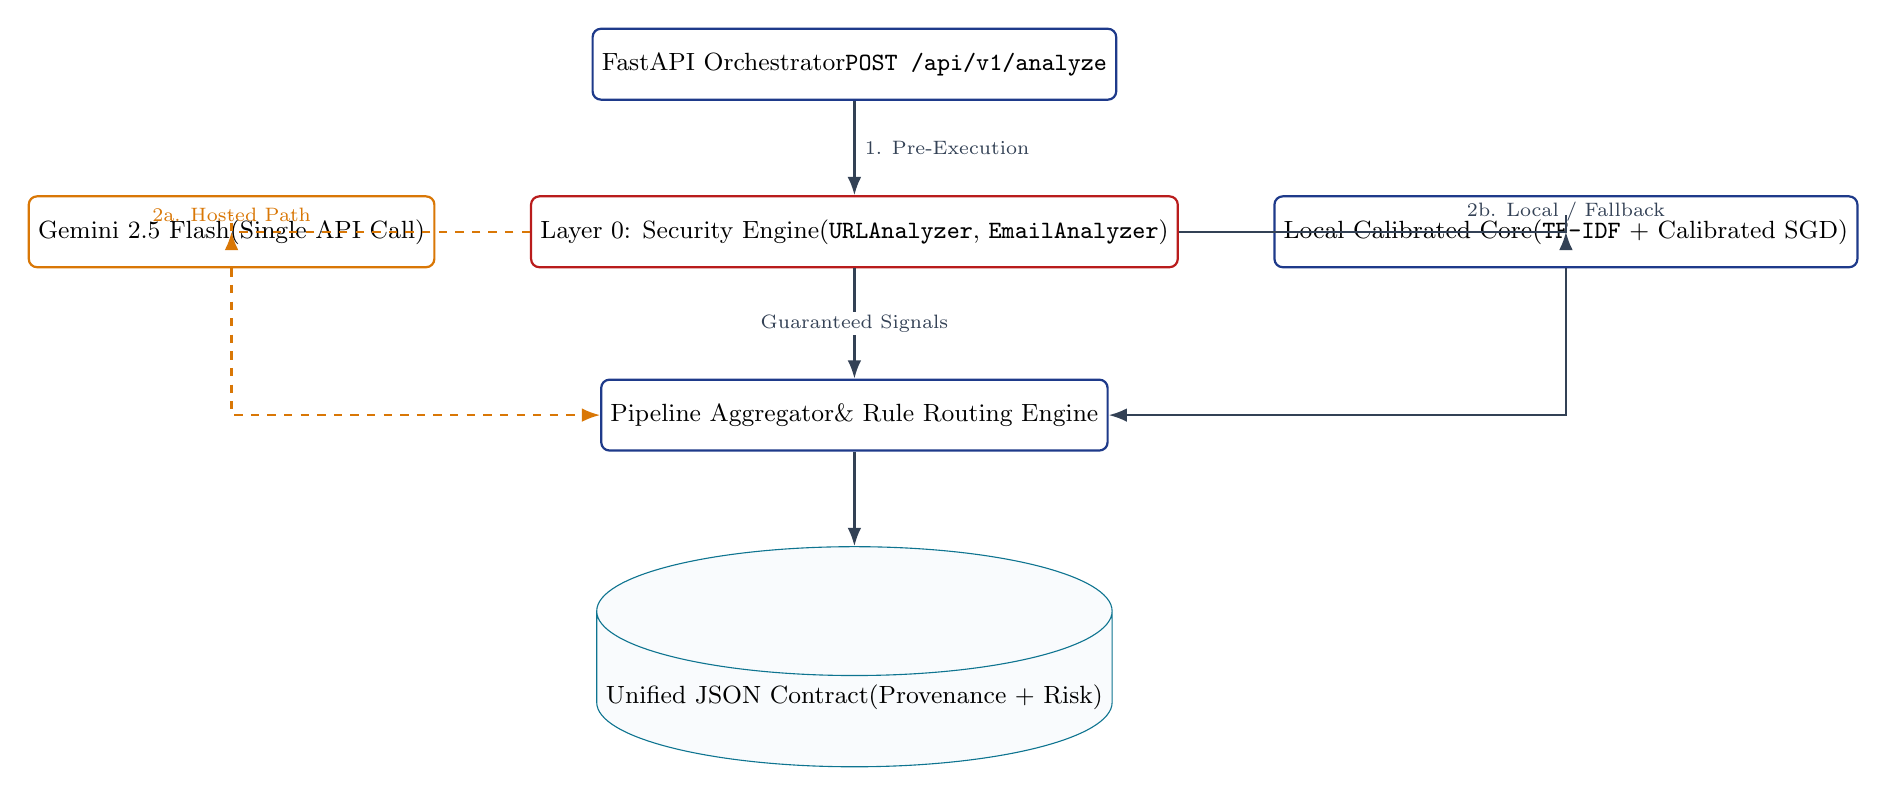
\begin{tikzpicture}[
    node distance=1.3cm and 1.5cm,
    box/.style={rectangle, draw=primary, fill=white, rounded corners=3pt, thick, text centered, minimum width=3.4cm, minimum height=0.9cm, font=\small},
    secbox/.style={rectangle, draw=danger, fill=white, rounded corners=3pt, thick, text centered, minimum width=3.4cm, minimum height=0.9cm, font=\small},
    geminibox/.style={rectangle, draw=accent, fill=white, rounded corners=3pt, thick, text centered, minimum width=3.4cm, minimum height=0.9cm, font=\small},
    databox/.style={cylinder, shape border rotate=90, draw=secondary, fill=lightgray!40, text centered, aspect=0.25, minimum width=2.6cm, minimum height=1.2cm, font=\small},
    arrow/.style={-Latex, thick, color=darkgray},
    dashedarrow/.style={-Latex, dashed, thick, color=accent}
]

    % Nodes
    \node[box] (api) {FastAPI Orchestrator \\ \texttt{POST /api/v1/analyze}};
    \node[secbox, below=1.2cm of api] (security) {Layer 0: Security Engine \\ (\texttt{URLAnalyzer}, \texttt{EmailAnalyzer})};
    
    \node[geminibox, left=1.2cm of security] (gemini) {Gemini 2.5 Flash \\ (Single API Call)};
    \node[box, right=1.2cm of security] (local) {Local Calibrated Core \\ (\texttt{TF-IDF} + Calibrated SGD)};
    
    \node[box, below=1.4cm of security] (features) {Pipeline Aggregator \\ \& Rule Routing Engine};
    
    \node[databox, below=1.2cm of features] (response) {Unified JSON Contract \\ (Provenance + Risk)};

    % Arrows
    \draw[arrow] (api) -- node[right, font=\scriptsize] {1. Pre-Execution} (security);
    \draw[dashedarrow] (security) -| node[above, font=\scriptsize] {2a. Hosted Path} (gemini);
    \draw[arrow] (security) -| node[above, font=\scriptsize] {2b. Local / Fallback} (local);
    \draw[dashedarrow] (gemini) |- (features);
    \draw[arrow] (local) |- (features);
    \draw[arrow] (security) -- node[fill=white, inner sep=1pt, font=\scriptsize] {Guaranteed Signals} (features);
    \draw[arrow] (features) -- (response);

\end{tikzpicture}
\caption{Solwin Dual-Tier Hybrid Intelligence Architecture.}
\label{fig:arch}
\end{figure}

% ==============================================================================
\section{Subsystem Decomposition \& Engineering Modules}
% ==============================================================================

\subsection{1. Deterministic Security Intelligence (\texttt{ml\_service.security})}
Security screening occurs \textbf{strictly prior} to any external generative AI call. Untrusted user text is treated as adversarial payload.
\begin{itemize}[leftmargin=*]
    \item \textbf{URL Threat Analyzer (\texttt{url\_analyzer.py}):}
    \begin{itemize}
        \item \textit{Punycode / Homograph Detection:} Identifies IDN spoofing via \texttt{xn--} prefixes mimicking authentic character sets.
        \item \textit{Direct IP Hostnames:} Flags raw IPv4/IPv6 hosts (\texttt{ipaddress.ip\_address}) avoiding domain reputation checks.
        \item \textit{Concealed Shorteners:} Detects domains (\texttt{bit.ly}, \texttt{tinyurl.com}, \texttt{t.co}) and mandates an automatic minimum risk penalty (\texttt{SecurityRiskLevel.MEDIUM}).
        \item \textit{Suspicious TLDs \& Credential Harvesting:} Evaluates risky TLDs (\texttt{.xyz}, \texttt{.top}, \texttt{.zip}) and path tokens (\texttt{/login}, \texttt{/verify}, \texttt{/invoice}, \texttt{.exe}) over unencrypted HTTP.
    \end{itemize}
    \item \textbf{Email \& Typosquatting Analyzer (\texttt{email\_analyzer.py}):}
    \begin{itemize}
        \item \textit{Levenshtein \& Replacement Lookalikes:} Matches domain tokens against authentic enterprise brands (Amazon, PayPal, Apple, Microsoft) to catch substitutions (\texttt{amaz0n}, \texttt{paypa1}, \texttt{micros0ft}).
        \item \textit{Synthetic Suffixes:} Flags domain strings like \texttt{paypal-security.com} or \texttt{amazon-support.net}.
        \item \textit{Disposable Providers:} Cross-references 25+ throwaway email providers (\texttt{tempmail}, \texttt{mailinator}).
    \end{itemize}
\end{itemize}

\subsection{2. Hierarchical Category Classification (\texttt{ml\_service.classification})}
Maps customer issues to 11 standard operational domains:
\begin{equation}
    \mathcal{C} = \{\text{PAYMENT\_TRANSACTION\_ISSUE}, \text{ACCOUNT\_LOGIN\_PROBLEM}, \dots, \text{SECURITY\_CONCERN}, \text{OTHER}\}
\end{equation}
The local model utilizes sublinear term frequency weighting over n-grams $(1, 2)$ fed into a calibrated ensemble with Platt probability calibration. An abstention threshold $\tau = 0.65$ automatically triggers \texttt{needs\_review = true} when uncertainty is elevated.

\subsection{3. Centroid Topic Clustering (\texttt{ml\_service.clustering})}
Enables unsupervised topic discovery across complaint queues. Uses KMeans with 15 optimized semantic cluster centroids. The distance metric:
\begin{equation}
    d(x, c_k) = \| \phi(x) - c_k \|_2
\end{equation}
computes distance to cluster centers, mapping incoming messages to top keywords and identifying emerging complaint topics in real-time.

\subsection{4. Objective Urgency \& Resolution Engines}
\begin{itemize}[leftmargin=*]
    \item \textbf{Urgency Engine (\texttt{ml\_service.urgency}):} Decouples angry sentiment from operational urgency. Detects financial loss, pending legal deadlines, and account takeover signals into \texttt{CRITICAL}, \texttt{HIGH}, \texttt{MEDIUM}, and \texttt{LOW}.
    \item \textbf{Resolution State Engine (\texttt{ml\_service.resolution}):} Factual status parser detecting delivery confirmations, refund completion, or ongoing blockages into \texttt{RESOLVED}, \texttt{UNRESOLVED}, or \texttt{PARTIALLY\_RESOLVED}.
\end{itemize}

\subsection{5. Deterministic Decision Engine (\texttt{ml\_service.recommendation})}
Evaluates multi-dimensional tuples:
\begin{equation}
    \mathcal{T} = \langle \text{Category}, \text{Urgency}, \text{ResolutionStatus}, \text{SecurityRisk} \rangle
\end{equation}
against declarative rules defined in \texttt{action\_rules.yaml}. Executes instant operational actions:
\begin{itemize}[leftmargin=*]
    \item \texttt{RULE\_SECURITY\_INCIDENT} $\longrightarrow$ Quarantine ticket, initiate credential freeze.
    \item \texttt{RULE\_PAYMENT\_FRAUD\_CRITICAL} $\longrightarrow$ Escalate to Tier 2 Payment Gateways.
    \item \texttt{RULE\_HIGH\_URGENCY\_RECOVERY} $\longrightarrow$ Route to Priority Support Desk.
\end{itemize}

% ==============================================================================
\section{Data Contracts \& Schema Specifications}
% ==============================================================================

The canonical interface between the Backend Orchestrator and the ML Service is governed by the schema below.

\subsection{Request Contract: \texttt{POST /api/v1/analyze}}
\begin{lstlisting}[language=json]
{
  "complaint_id": "CMP-2026-9901",
  "complaint": {
    "subject": "Unauthorized card charge and suspicious verification link",
    "message": "I was charged $450 twice. SMS linked to http://192.168.1.1/verify."
  },
  "include_cluster": true,
  "include_urgency": true,
  "include_resolution": true,
  "include_recommendation": true,
  "include_security": true,
  "include_summary": true,
  "prefer_llm": false
}
\end{lstlisting}

\subsection{Response Contract}
\begin{lstlisting}[language=json]
{
  "complaint_id": "CMP-2026-9901",
  "classification": {
    "category": "PAYMENT_TRANSACTION_ISSUE",
    "confidence": 0.961,
    "needs_review": false,
    "model_name": "gemini-2.5-flash"
  },
  "cluster": {
    "cluster_id": 3,
    "cluster_name": "Payment & Transaction Failures",
    "distance": 0.384,
    "keywords": ["charge", "deducted", "verify", "gateway"]
  },
  "urgency": {
    "urgency": "HIGH",
    "confidence": 0.88,
    "signals": ["monetary_deduction", "unauthorized_transaction"]
  },
  "resolution": {
    "status": "UNRESOLVED",
    "confidence": 0.90
  },
  "security": {
    "aggregate_risk": "HIGH",
    "requires_quarantine": true,
    "risk_reasons": ["ip_address_host", "suspicious_path_keywords:verify"],
    "urls": [{
      "url": "http://192.168.1.1/verify",
      "risk_level": "HIGH",
      "risk_score": 0.70
    }]
  },
  "recommendation": {
    "primary_action": "ESCALATE_TO_SECURITY_TEAM",
    "matched_rule_id": "RULE_CRITICAL_SECURITY_ESCALATION"
  },
  "processing_time_ms": 4.12
}
\end{lstlisting}

% ==============================================================================
\section{Resilience, Failover \& Performance Guarantees}
% ==============================================================================

\begin{table}[htbp]
\centering
\small
\begin{tabularx}{\linewidth}{l X l}
\toprule
\textbf{Condition / Fault} & \textbf{Mitigation Strategy} & \textbf{Fallback Target} \\
\midrule
\textbf{Gemini API Rate Limit (429)} & Circuit breaker catches error, logs warning & Local TF-IDF Classifier \\
\textbf{Gemini Timeout ($> 10$s)} & Non-blocking client deadline termination & Local Urgency \& Heuristics \\
\textbf{Malformed Customer Input} & Sanitizer strips control chars \& normalizes & Extractive Fallback Engine \\
\textbf{Malicious Link Insertion} & Deterministic Layer 0 regex intercepts link & Ticket auto-quarantine \\
\textbf{PII / Secret Exposure} & Safe logging recursively redacts PANs, keys & Clean structured logs \\
\bottomrule
\end{tabularx}
\caption{System Resilience \& Fallback Matrix.}
\label{tab:resilience}
\end{table}

\subsection{Latency Profile}
\begin{itemize}[leftmargin=*]
    \item \textbf{Deterministic Path (CPU):} $\leq 5\text{ms}$ at 99th percentile ($p99$).
    \item \textbf{Hybrid Gemini Path (Network Bound):} $450\text{ms} - 800\text{ms}$ ($p95$).
    \item \textbf{Container Footprint:} $\approx 180\text{MB}$ Resident Set Size (RSS), lightweight Alpine Linux base.
\end{itemize}

% ==============================================================================
\section{Conclusion \& Verification Instructions}
% ==============================================================================
The Solwin ML Services architecture satisfies all production requirements: strict separation of concerns, guaranteed defensive screening, low-latency execution, and resilient graceful degradation.

To compile this document in Overleaf:
\begin{enumerate}[leftmargin=*]
    \item Create a new blank project on \href{https://www.overleaf.com}{Overleaf}.
    \item Paste this file content into \texttt{main.tex}.
    \item Ensure compiler is set to \textbf{pdfLaTeX} (default).
    \item Click \textbf{Recompile}.
\end{enumerate}

\end{document}
